{
\catcode`\%=12
\begin{table}[]
\begin{tabular}{cll}
\multicolumn{1}{l}{\textbf{Morph}}               & \textbf{Description} & \textbf{Snapshot} \\
\cellcolor[HTML]{4C72B0}{\color[HTML]{FFFFFF} a} &  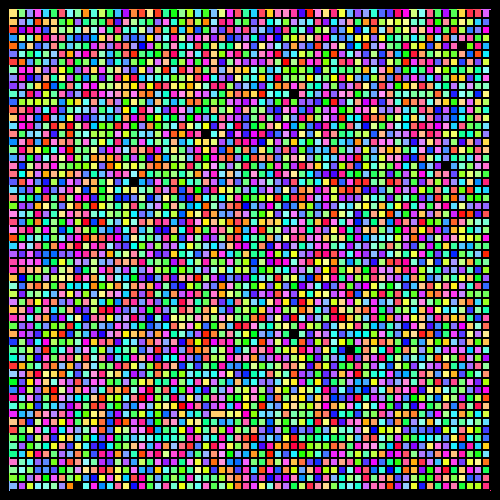
\includegraphics[width=\linewidth]{\detokenize{snapshots/a=kin-group-id+idx=0+proc=0+series=16005+stint=0+thread=0+update=28991+_endeavor=16+_repro=rvV3h5Ru0tlNBvox+_slurm_job_id=24414678+_source=8eb7a4e-dirty+_treatment=bucket%prq49~diversity%0.50_series~mut_freq%1.00~mut_sever%1.00+ext=}}             & todo              \\
\cellcolor[HTML]{DD8452}{\color[HTML]{FFFFFF} b} & todo                 & todo              \\
\cellcolor[HTML]{55A868}{\color[HTML]{FFFFFF} c} & todo                 & todo              \\
\cellcolor[HTML]{C44E52}{\color[HTML]{FFFFFF} d} & todo                 & todo              \\
\cellcolor[HTML]{8172B3}{\color[HTML]{FFFFFF} e} & todo                 & todo              \\
\cellcolor[HTML]{937860}{\color[HTML]{FFFFFF} f} & todo                 & todo              \\
\cellcolor[HTML]{DA8BC3}{\color[HTML]{FFFFFF} g} & todo                 & todo              \\
\cellcolor[HTML]{8C8C8C}{\color[HTML]{FFFFFF} h} & todo                 & todo              \\
\cellcolor[HTML]{CCB974}{\color[HTML]{FFFFFF} i} & todo                 & todo              \\
\cellcolor[HTML]{64B5CD}{\color[HTML]{FFFFFF} j} & todo                 & todo             
\end{tabular}
\end{table}
}